\chapter{FUNDAMENTAÇÃO TEÓRICA}

Para melhor compreender as decisões de projeto tomadas durante o desenvolvimento da proposta deste trabalho é necessário entender alguns conceitos teóricos relacionados a robôs móveis e ROS.


\section{\textit{ROBÔS MÓVEIS}}

De acordo com \citeonline{niloy2021critical} "Robôs que podem se mover de forma autônoma e podem tomar decisões inteligentes percebendo seus ambientes e objetos ao redor são conhecidos como robôs móveis autônomos". Um dos primeiros exemplos disso é o robô \textit{Tortoise}, ilustrado na Figura \ref{fig:tortoise}, criado por W. Grey Walter.

\begin{figure}[!ht]
  \caption{\label{fig:tortoise}"Tortoise" robô móvel}
  \centering
  \includegraphics[scale=0.8]{figuras/tortoise.pdf}
  \legend{\Fonte{\cite{9014460}.}}
\end{figure}


O \textit{Tortoise} foi projetado com dois sensores. O primeiro é uma célula fotoelétrica, que consiste em um dispositivo que produz um sinal elétrico como resposta à exposição à radiação eletromagnética. Essa célula rotacionava e funcionava como o ``olho'' da máquina, varrendo os arredores até encontrar uma fonte de luz. O robô parava de escanear e andava em direção a fonte de luz ou, se a fonte fosse muito forte, se distanciava dela. O segundo é um interruptor de contato externo, sensível ao toque. Que faz o robô recuar quando encontra obstáculos. O \textit{Tortoise} retorna à base de carregamento quando sua bateria está baixa.

Robôs móveis de interior são projetados para se mover, correr ou andar para poderem completar suas tarefas específicas, então podem ser equipados com pernas, rodas ou até mesmo asas (os que possuem rodas se provam os mais eficientes, como será demonstrado na sessão seguinte) \cite{dubey2015robot}. Neste trabalho o foco será um robô móvel de interior movido por rodas.


\subsection{Locomoção por rodas}

Em consoante com \citeonline{nicolino_de_sa_modelagem_2016}, a locomoção por rodas é um dos mecanismos mais utilizados por ser o método mais simples de deslocamento para robôs móveis já que ele é usado em vários veículos no geral. Por conta da estabilidade, fácil controle e o design mecânico relativamente simples o uso de rodas é bem eficiente e de fácil implementação.

Ainda de acordo com \citeonline{nicolino_de_sa_modelagem_2016}, a seleção do tipo de rodas para um robô móvel está intrinsecamente relacionada à disposição e geometria das rodas na estrutura robótica, sendo crucial considerar esses dois aspectos no planejamento do sistema de deslocamento. Estas escolhas afetam diretamente três características essenciais de um robô: estabilidade, capacidade de manobra e capacidade de controle.

Diante disso, existem 4 tipos diferentes de locomoção por rodas, sendo eles:

\begin{itemize}
    \item[\textbf{a)}] \textbf{Roda padrão:} dois graus de liberdade e a rotação ao redor do eixo e ponto de contato.
    
    \item[\textbf{b)}] \textbf{Roda rodízio:} dois graus de liberdade e o giro ocorre ao redor da junta de direção deslocada.
    
    \item[\textbf{c})] \textbf{Roda omnidirecional:} três graus de liberdade e a rotação ocorre ao redor dos rolos, eixo da roda e do ponto de contato.
    
    \item[\textbf{d)}] \textbf{Roda esférica:} tem mais área superficial que a roda de rodízio que é cilíndrica.
\end{itemize}

A Figura \ref{fig:rodas} mostra as quatro categorias de rodas utilizadas em robôs móveis. Dependendo do ambiente o arranjo de rodas pode utilizar mais de um tipo ou várias de um mesmo tipo. Tanto o tipo de roda, quanto a geometria são características fundamentais no funcionamento do robô determinando a manobrabilidade, controlabilidade e estabilidade.


\begin{figure}[!ht]
  \caption{\label{fig:rodas}Os quatro tipos de rodas.}
  \centering
  \includegraphics[scale=0.4]{figuras/tipos_de_rodas.pdf}
  \legend{\Fonte{\cite{siegwart2011introduction}.}}
\end{figure}

Embora rodas omnidirecionais e esféricas permitam maior liberdade de movimento e holonomia, elas exigem mecanismos mais complexos e maior manutenção. Para o presente trabalho, a combinação de rodas padrão (tração) com roda rodízio (apoio) foi selecionada por oferecer a robustez necessária para um robô seguidor de linha, onde a precisão da trajetória é priorizada em detrimento da capacidade de deslocamento lateral. A Figura \ref{fig:rodas} ilustra essas categorias.

\subsection{Cinemática Diferencial}
\label{subsec:cinematica_diferencial}

A plataforma robótica que será desenvolvida neste trabalho utiliza uma configuração de acionamento diferencial, que consiste em duas rodas motrizes montadas em um eixo comum, cada uma controlada independentemente por seu próprio motor, e uma roda passiva (\textit{caster}) para equilíbrio e estabilidade. Segundo \citeonline{siegwart2011introduction}, esta é uma das configurações mais comuns em robótica móvel devido à sua simplicidade mecânica e capacidade de girar no próprio eixo (raio de giro zero).

A cinemática deste sistema descreve a relação entre as velocidades das rodas e a velocidade do robô no espaço global. Diferente de veículos omnidirecionais, que podem se mover em qualquer direção instantaneamente, um robô diferencial está sujeito a restrições não-holonômicas, o que significa que ele não pode se deslocar lateralmente sem antes realizar uma rotação \cite{lynch2017modern}.

Dessa maneira, para modelar o movimento, considera-se $v_L$ e $v_R$ como as velocidades lineares das rodas esquerda e direita, respectivamente. A velocidade linear $v$ do robô e sua velocidade angular $\omega$ em torno do centro do eixo são dadas pelas Equações \ref{eq:cinematica_v} e \ref{eq:cinematica_w}, onde $L$ representa a distância entre as rodas (\textit{track width}):

\begin{equation}
    v = \frac{v_R + v_L}{2}
    \label{eq:cinematica_v}
\end{equation}

\begin{equation}
    \omega = \frac{v_R - v_L}{L}
    \label{eq:cinematica_w}
\end{equation}

Sob esta óptica, essas equações compõem a cinemática direta, utilizada para calcular a odometria do robô. No contexto do controle de navegação, no entanto, é frequentemente necessário o processo inverso: determinar a velocidade de rotação necessária para cada motor a partir de uma velocidade linear e angular desejada. A cinemática inversa é expressa por:

\begin{equation}
    v_R = v + \frac{\omega \cdot L}{2}
    \label{eq:inversa_vr}
\end{equation}

\begin{equation}
    v_L = v - \frac{\omega \cdot L}{2}
    \label{eq:inversa_vl}
\end{equation}

Ademais, estudos recentes, como o de \citeonline{ferreira2023differential}, demonstram que a precisão deste modelo cinemático é fundamental para minimizar erros de trajetória em ambientes reais, onde fatores como escorregamento das rodas e irregularidades do piso podem introduzir incertezas que devem ser compensadas por malhas de controle, como o PID implementado neste projeto.

\section{\textit{ROS}}

\textit{Robot Operating System} (ROS) ou Sistema Operacional Robótico é um kit de desenvolvimento de software de código aberto para aplicações de robótica. Ele oferece uma plataforma de software padrão para desenvolvedores de todos os setores que os levarão desde a pesquisa e a prototipagem até a implantação e a produção \cite{ROS.org}. ROS é um sistema de código aberto e meta-operacional, que provê os serviços que você normalmente espera de um sistema operacional, tais como \citeonline{macenski2022robot}, \citeonline{quigley2009ros} e \citeonline{koubaa2017robot}:
\begin{itemize}
    \item abstração de hardware;
    \item controle de dispositivo de baixo nível;
    \item implementação de funcionalidade comumente usada;
    \item troca de mensagens entre processos;
    \item gerenciamento de pacotes.
\end{itemize}

O ROS é o sistema operacional destinado a sistemas robóticos, permite comunicar softwares que utilizam diferentes linguagens de programação, bem como ligar os diferentes dispositivos de entrada ou saída de forma trivial e, além desta particularidade, reúne os esforços de vários desenvolvedores nesta área \cite{quigley2015programming}. São mais de 7000 pacotes desenvolvidos para as várias distribuições do ROS \cite{ROSindex}. Por mais de 10 anos, o projeto ROS produziu um vasto ecossistema de software para robótica, alimentando uma comunidade global de milhões de desenvolvedores e usuários que contribuem e melhoram esse software \cite{WhyRos}.

Mesmo que houvesse pesquisas de robótica acontecendo antes do ROS, a maior parte do software era exclusiva para seus próprios robôs. Seu software pode ser de código aberto, mas é muito difícil de reutilizar. Comparando o ROS com sistemas robóticos existentes, ele desempenha bem melhor nos seguintes aspectos \cite{joseph2017ros}:

\begin{itemize}
    \item \textbf{Desenvolvimento colaborativo}: Como discutido, o ROS é de código aberto e gratuito para uso em indústrias e pesquisas. Os desenvolvedores podem expandir as funcionalidades do ROS adicionando pacotes. Quase todos os pacotes de ROS funcionam em uma camada de abstração de hardware, portanto, podem ser reutilizados facilmente para outros robôs.
    
    \item \textbf{Suporte a linguagem}: O \textit{framework} de comunicação ROS pode ser facilmente implementado em qualquer linguagem moderna. Ele já suporta linguagens populares como C++ e Python, e possui bibliotecas que são mantidas por membros da comunidade que dão suporte a linguagens como Ada, C, Node.js, Rust, entre outras.
    
    \item \textbf{Integração de bibliotecas}: O ROS possui uma interface para muitas bibliotecas robóticas de terceiros, como \textit{Open Source Computer Vision} (Open-CV), \textit{Point Cloud Library} (PCL), Open-NI, Open-Rave e Orocos. Os desenvolvedores podem trabalhar com qualquer uma dessas bibliotecas sem muito trabalho.
    
    \item \textbf{Integração de simuladores}: O ROS também está vinculado a simuladores de código aberto, como Gazebo e Webots, e possui uma boa interface com simuladores proprietários, como CoppeliaSim.
    
    \item \textbf{Teste de código}: O ROS oferece uma estrutura de teste embutida chamada rostest para verificar a qualidade do código e \textit{bugs}.
    
    \item \textbf{Escalabilidade}: A estrutura ROS foi projetada para ser escalonável. Pode-se realizar tarefas de grande custo computacional com robôs usando ROS, que podem ser colocados na nuvem ou em \textit{clusters} heterogêneos.
    
    \item \textbf{Customização}: Conforme discutido, o ROS é totalmente de código aberto e gratuito, portanto, pode-se personalizar essa estrutura de acordo com os requisitos do robô. Se quisermos apenas trabalhar com a plataforma de mensagens ROS, podemos remover todos os outros componentes e usar apenas isso. Pode-se até personalizar o ROS para um robô específico para melhor desempenho.
    
    \item \textbf{Comunidade}: O ROS é um projeto voltado para a comunidade, liderado principalmente pela \textit{Open Source Robotics Foundation} (OSRF). O grande apoio da comunidade é uma grande vantagem para o ROS, e pode-se facilmente iniciar o desenvolvimento de aplicativos de robótica.
\end{itemize}

Sob esse panorama, em razão de todas as vantagens presentes explicitadas, o ROS é um dos principais \textit{frameworks} e essencialmente é aplicado no desenvolvimento de sistemas robóticos e de automação ao redor do mundo.


\subsection{Conceitos básicos}

O \textit{node} é uma unidade de código executável, ele troca informação com outros \textit{nodes} através de \textit{messages} formando um grande programa. O conceito chave é o método de comunicação por \textit{message} entre os \textit{nodes}. A conveniência é que cada \textit{node} executa um simples propósito, para facilitar a reusabilidade e o desenvolvimento \cite{ROS_book_En}.

Um \textit{package} é unidade básica do ROS. As aplicações do ROS são desenvolvidas baseadas em \textit{packages}, ele contém os arquivos de configuração para executar outros \textit{packages} ou \textit{nodes}. O \textit{package} também contém todos os arquivos necessários para execução, incluindo bibliotecas de dependência do ROS para executar vários processos \cite{ROS_book_En}. Por exemplo, o ROS kinect que foi a distribuição mais popular por bastante tempo, conta com uma biblioteca com 2772 \textit{packages} \cite{ROSindex}.

A \textit{message} é um conjunto de dados que são enviados e recebidos pelos \textit{nodes}. \textit{Messages} possuem variáveis como inteiros, floats e booleanos. Uma \textit{message} pode ser estruturada contendo várias outras \textit{messages} dentro dela.

Os \textit{topics} são um elemento vital do gráfico ROS que atuam como um barramento para os \textit{nodes} trocarem \textit{messages}. Um \textit{node} pode publicar dados para qualquer número de \textit{topics} e, simultaneamente, ter assinaturas para qualquer número de \textit{topics}.

O \textit{service} é a comunicação bidirecional síncrona entre o cliente de serviço que solicita um serviço referente a uma tarefa específica e o servidor de serviço que é responsável por responder às solicitações.

As \textit{actions} são um dos tipos de comunicação, exclusivas do ROS 2, são destinadas a tarefas de longa duração. Eles consistem em três partes: uma meta, retorno e um resultado. As \textit{actions} são construídas em \textit{topics} e \textit{services}. Sua funcionalidade é semelhante à dos \textit{services}, exceto que as \textit{actions} são preemptivas (é possível cancelá-las durante a execução). Eles também fornecem retorno constante, ao contrário de \textit{services} que retornam uma única resposta.

O \textit{namespace} é um mecanismo para encapsular grupos de execução no ROS. É bastante útil quando é necessário executar mais de uma vez o mesmo \textit{node} e separar as informações entre eles, evitando conflitos de nomes.

Sob esse viés, é explicitado na Figura \ref{fig:node} o diagrama de comunicação entre \textit{nodes} através de \textit{topics} e \textit{services} dentro do ambiente do ROS.


\begin{figure}[!ht]
  \caption{\label{fig:node}Comunicação entre \textit{nodes}.}
  \centering
  \includegraphics[scale=0.55]{figuras/estrutura_node.pdf}
  \legend{\Fonte{\cite{RosDocs}.}}
\end{figure}


Atualmente o ROS está na sua segunda versão, o ROS 2. Normalmente quando o termo ROS é citado está sendo referenciado a comunidade e o projeto como um conceito geral. Para diferenciar as versões será utilizado o termo ROS 1 e ROS 2 quando for necessário apontar características específicas de cada um. A principal diferença entre as duas versões é a arquitetura de como é feita a comunicação entre os \textit{nodes}. No ROS 1 era necessário ter um \textit{node} chamado \textit{Master} que gerenciava as comunicações e utilizava o protocolo TCP/UDP para comunicação. No ROS 2 isso é feito na camada de \textit{middleware} e o protocolo é o \textit{Data Distribution Service} (DDS) \cite{inproceedings}, como mostrado na Figura \ref{fig:dif1&2}.


\begin{figure}[!ht]
  \caption{\label{fig:dif1&2}Arquitetura ROS 1/ROS 2.}
  \centering
  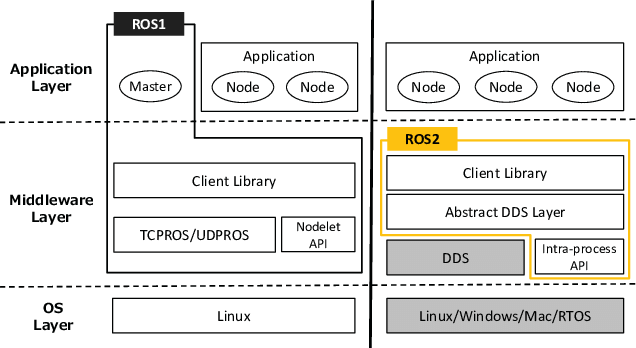
\includegraphics[scale=0.6]{figuras/ROS1-ROS2-architecture-for-DDS-approach-to-ROS-We-clarify-the-performance-of-the-data.png}
  \legend{\Fonte{\cite{inproceedings}.}}
\end{figure}


\subsection{Casos de uso}

Recentemente foi divulgada uma lista pública com quase 400 empresas conhecidas que utilizam o ROS 1 ou ROS 2, ou qualquer de suas ferramentas de desenvolvimento, para criar produtos ou oferecer serviços. Nessa lista constam desde empresas centenárias como a Bosch, Boeing, BMW Group, Jhon Deere, KUKA, até empresas recentes Toyota Woven Planet, TechnoYantra, Tangram Vision, Stogl Robotics \cite{roscomp}. Inclusive, algumas delas trabalham especificamente prestando consultoria do uso de ROS.

Nesse contexto, em ambientes terrestres, \citeonline{miller2020mine} apresenta em sua pesquisa a utilização de múltiplos robôs quadrúpedes da empresa Ghost Robotics para a exploração em túneis de minas subterrâneas (Figura \ref{fig:miller}). O ROS foi incorporado ao sistema, dando suporte ao controle da missão, permitindo o mapeamento e retorno. Durante a missão, o sistema identifica e cruza informações com o banco de dados, em seguida é possível montar e executar cada ação necessária, isso tudo através de \textit{Application Programming Interfaces} (API) que se utilizam da interface \textit{publisher-subscriber}.


\begin{figure}[!ht]
  \caption{\label{fig:miller}Robôs quadrúpedes para exploração e mapeamento em minas subterrâneas.}
  \centering
  \includegraphics[scale=0.4]{figuras/Miller.pdf}
  \legend{\Fonte{\cite{miller2020mine}.}}
\end{figure}


Como outro exemplo de destaque, pode-se citar a \textit{National Aeronautics and Space Administration} (NASA), que possui uma missão chamada \textit{Volatiles Investigating Polar Exploration Rover} (VIPER), com o intuito de explorar a região polar da lua e buscar gelo e outros recursos. Várias das ferramentas de operações baseadas na Terra, módulos de cálculo e simulações de alta fidelidade são baseadas no ROS 2 e Gazebo. Como mostrado na Figura \ref{fig:viper_nasa}, em "A" temos o robô \textit{VIPER} na superfície da lua (renderizado), e em "B" o \textit{software} de operação e comandos, conforme \citeonline{macenski2022robot}.


\begin{figure}[!ht]
  \caption{\label{fig:viper_nasa}Robô VIPER da NASA.}
  \centering
  \includegraphics[scale=0.28]{figuras/viper_nasa.pdf}
  \legend{\Fonte{\cite{macenski2022robot}.}}
\end{figure}


\subsection{Micro-ROS}

De acordo com \citeonline{MicroRos} a missão do time que desenvolve o micro-ROS é preencher o espaço entre microcontroladores com recursos restritos e processadores mais potentes em aplicações robóticas que são baseadas no ROS. Com o micro-ROS é possível fazer com que microcontroladores, mais baratos e simples que computadores e notebooks, utilizem o ROS. Esses microcontroladores são usados em quase todos os robôs, os principais motivos são o acesso ao hardware, baixa latência e economia de energia. 

O micro-ROS segue a arquitetura do ROS 2 e toma proveito da capacidade de conexão do \textit{middleware} para utilizar \textit{Data Distribuiton Service - Extremely Resource Constrained Environments} (DDS-XRCE), que é otimizado para microcontroladores. Entretanto ele utiliza o \textit{Real Time Operating System} (RTOS) baseado em \textit{Portable Operating System Interface} (POSIX) ao invés de Linux.

A Figura \ref{fig:microros} demonstra como funciona a arquitetura do micro-ROS. Em azul escuro estão os componentes desenvolvidos especificamente para o micro-ROS. Azul claro são os componentes padrões do ROS 2 que foram utilizados. O ROS 2 \textit{Agent} é o nó responsável por fazer a ponte de comunicação entre o microcontrolador e o computador com mais poder de processamento. 


\begin{figure}[!ht]
  \caption{\label{fig:microros}Arquitetura do micro-ROS.}
  \centering
  \includegraphics[scale=1.4]{figuras/micro-ROS_architecture.pdf}
  \legend{\Fonte{\cite{MicroRos}.}}
\end{figure}


\section{ESP-32}

O ESP32, exposto na Figura \ref{fig:esp32}, é uma série de microcontroladores SOC (\textit{System On Chip} – Sistema em um
Chip), desenvolvidos pela empresa chinesa Espressif Systems. É composto
por um módulo Wi-Fi com conectividade 802.11b/g/n e Bluetooth de modo duplo integrados em
sua placa de desenvolvimento, imprescindível para aplicações em IoT  \cite{babiuch2019using}.


\begin{figure}[!ht]
  \caption{\label{fig:esp32}Microcontrolador ESP-32.}
  \centering
  \includegraphics[scale=0.4]{figuras/esp32.pdf}
  \legend{\Fonte{Retirada da Internet.}}
\end{figure}


Este microcontrolador, da segunda geração de microcontroladores com soluções IoT, fabricados pela Espressif, estabelece-se como sucessor direto do microcontrolador ESP8266. Esta série de microcontroladores compõe um microprocessador Xtensa LX6, fabricado pela empresa Tensilica, com arquitetura de 32 bits, em duas versões: de 1 ou 2 núcleos (single-core ou dualcore). A velocidade de clock é de até 240 MHz, com 520 KB de SRAM (\textit{Static Random Access Memory} – Memória de Acesso Aleatório Estático)\cite{dokic2020microcontrollers}.

Além de contar com um módulo Wi-Fi mais rápido e com maior alcance, em comparação ao ESP-8266, em consoante com \citeonline{rodrigues2024internet}, este microcontrolador possui também suporte para duas versões Bluetooth, versão 4.2 e BLE (\textit{Bluetooth Low Energy}). Para mais, o ESP32 ainda conta com mais canais de entrada e saída (GPIO), conforme a Tabela \ref{tab:especificacoes_esp32_esp8266}, que apresenta uma comparação entre o ESP8266 e o ESP32.


\begin{table}[!ht]
\Caption{\label{tab:especificacoes_esp32_esp8266}Especificações do ESP8266 e ESP32.}
\resizebox{\linewidth}{!}{
\begin{tabular}{|c|c|c|}
  \hline
  \textbf{Especificação} & \textbf{ESP8266} & \textbf{ESP32}\\
  \hline
   Wifi 802.11b/g/n & 2.4GHz, 72.2 Mbps & 2.4GHz, 150 Mbps \\
   \hline 
   Bluetooth & Não suporta & Bluetooth v4.2 e Bluetooth LE \\
   \hline 
   CPU & Xtensa L106 de 1 núcleo & Xtensa LX6 de 1 ou 2 núcleos \\
   \hline 
   Arquitetura & 32 bits & 32 bits \\
   \hline 
   Frequência do Clock & 80 MHz & 160 a 240 MHz \\
   \hline 
   Memória RAM & 50 KB RAM & 520 KB SRAM \\
   \hline 
   Memória ROM & Não suporta & 448 KB ROM \\
   \hline 
   Memória Flash & 512 KB & 4 MB \\
   \hline 
   GPIO & 17 canais & 36 canais \\
   \hline 
   Conversor AD & 1 canal de 10 bits & 18 canais de 12 bits \\
   \hline 
   Conversor DA & Não suporta & 2 canais de 8 bits \\
   \hline 
   SPI/I2C/I2S/UART
(Serial)
 & 2/1/2/2 canais & 4/2/2/2 canais \\
   \hline 
   PWM & 8 canais & 16 canais \\
   \hline 
   Sensor de toque capacitivo & Não suporta & 10 canais \\
  \hline
\end{tabular}}
\Fonte{\cite{rodrigues2024internet}.}
\end{table}


Sob esse panorama, esse módulo é amplamente utilizada em projetos de Internet das coisas (IoT), conforme apresentado por \citeonline{rodrigues2023aplicaccoes},  bem como outros projetos.


\section{Raspberry Pi 4 Model B}

O Raspberry Pi 4 Model B, ilustrado na Figura 9, é um computador de placa única (Single Board Computer - SBC) desenvolvido pela Raspberry Pi Foundation. Caracterizado por seu alto desempenho e baixo custo, ele é amplamente utilizado em projetos de computação embarcada, automação e robótica. Este modelo conta com um processador ARM Cortex-A72 quad-core de 64 bits rodando a 1,5 GHz, que oferece uma capacidade de processamento significativamente superior às versões anteriores. Além disso, dispõe de múltiplas opções de memória RAM, que vão de 2 GB a 8 GB, permitindo flexibilidade para diferentes aplicações \cite{rpi4}


\begin{figure}[!ht]
  \caption{\label{fig:rpi4}Raspberry Pi 4 Model B.}
  \centering
  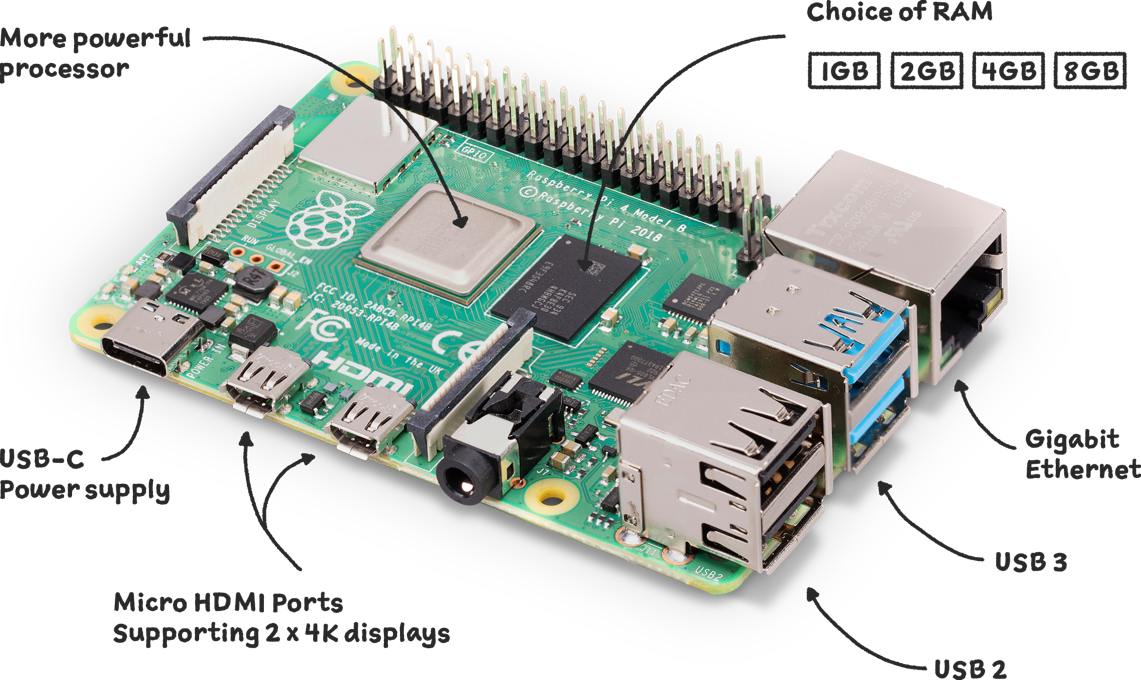
\includegraphics[scale=0.4]{figuras/raspberry-pi-4.png}
  \legend{\Fonte{\cite{rpi4}}}
\end{figure}


Este SBC oferece conectividade completa com interfaces como USB 3.0, USB 2.0, Gigabit Ethernet, Bluetooth 5.0 e Wi-Fi 802.11ac, com \textit{throughput} maior que plataformas como Arduino \cite{rpi_network_throughput}, o que é fundamental para projetos de Internet das Coisas (IoT) e robótica, onde a comunicação eficiente é essencial. A capacidade de suportar até duas saídas de vídeo 4K e múltiplas interfaces GPIO (General Purpose Input/Output) permite o controle direto de sensores, atuadores e outros dispositivos eletrônicos, favorecendo o desenvolvimento de sistemas integrados e plataformas robóticas avançadas.
